\documentclass{standalone}

\usepackage{amsmath}
\usepackage{tikz}
\usetikzlibrary{arrows.meta, positioning, calc, patterns}

\renewcommand{\familydefault}{\rmdefault}
\usepackage[T1]{fontenc}
\usepackage{lmodern}

\begin{document}

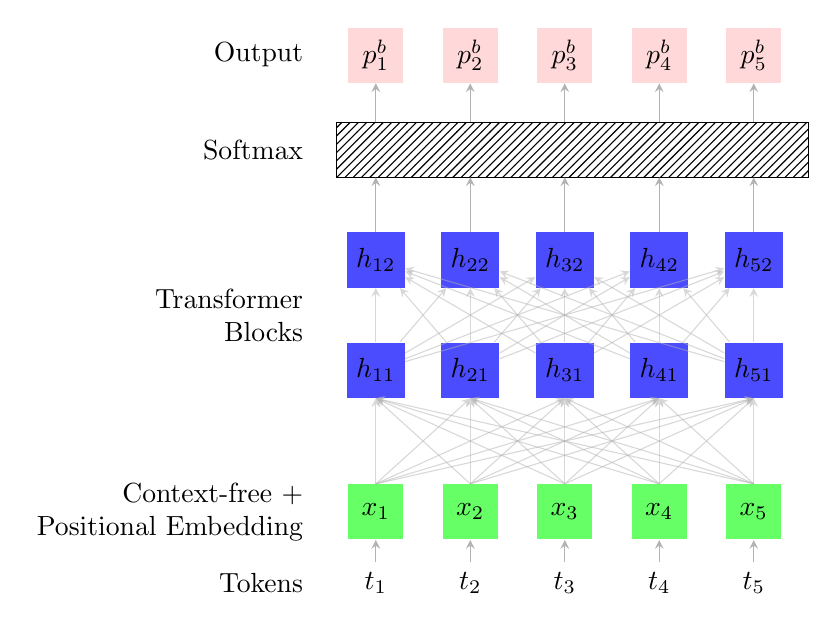
\begin{tikzpicture}[
    >=stealth,
    embed/.style={rectangle, fill=green!60, minimum size=7mm},
    hidden/.style={rectangle, fill=blue!70, minimum size=7mm},
    output/.style={rectangle, fill=pink!60, minimum size=7mm},
    conn/.style={gray!60,->,thin}
]

% -------- Layout --------
\def\xstart{0}
\def\xgap{1.2}

\def\yembed{0}
\def\yhOne{1.8}
\def\yhTwo{3.2}
\def\ysoft{4.6}
\def\yout{5.8}

% -------- Left labels (closer) --------
\node[left] at (-0.8,\yout) {Output};
\node[left] at (-0.8,\ysoft) {Softmax};
\node[left, align=right] at (-0.8,2.5) {Transformer\\Blocks};
\node[left, align=right] at (-0.8,\yembed) {Context-free +\\Positional Embedding};
\node[left] at (-0.8,-0.9) {Tokens};

% -------- Tokens + embeddings --------
\foreach \i in {1,...,5} {
    \pgfmathsetmacro{\x}{\xstart + (\i-1)*\xgap}

    \node (t\i) at (\x,-0.9) {$t_{\i}$};
    \node[embed] (x\i) at (\x,\yembed) {$x_{\i}$};

    \draw[conn] (t\i.north) -- (x\i.south);
}

% -------- Hidden layers --------
\foreach \i in {1,...,5} {
    \pgfmathsetmacro{\x}{\xstart + (\i-1)*\xgap}

    \node[hidden] (h\i1) at (\x,\yhOne) {$h_{\i 1}$};
    \node[hidden] (h\i2) at (\x,\yhTwo) {$h_{\i 2}$};
}

% -------- Embedding → first layer (FULL attention) --------
\foreach \i in {1,...,5} {
    \foreach \j in {1,...,5} {
        \draw[conn, opacity=0.5] (x\i.north) -- (h\j1.south);
    }
}

% -------- Layer 1 → Layer 2 (FULL attention) --------
\foreach \i in {1,...,5} {
    \foreach \j in {1,...,5} {
        \draw[conn, opacity=0.5] (h\i1) -- (h\j2);
    }
}

% -------- Softmax --------
\draw[pattern=north east lines]
    (-0.5,\ysoft-0.35) rectangle (5*\xgap-0.5,\ysoft+0.35);

% -------- Outputs --------
\foreach \i in {1,...,5} {
    \pgfmathsetmacro{\x}{\xstart + (\i-1)*\xgap}

    \node[output] (p\i) at (\x,\yout) {$p^b_{\i}$};

    \draw[conn] (h\i2.north) -- (\x,\ysoft-0.35);
    \draw[conn] (\x,\ysoft+0.35) -- (p\i.south);
}

\end{tikzpicture}
\hspace{1em}

\end{document}